\documentclass[11pt]{article}
\usepackage{amsmath,amssymb,array,booktabs,longtable,geometry,fontspec}
\usepackage{tikz}\usetikzlibrary{arrows.meta}
\usepackage[hidelinks]{hyperref}
\geometry{margin=1in}
\setlength{\emergencystretch}{3em}
\frenchspacing
\IfFontExistsTF{Times New Roman}
  {\setmainfont{Times New Roman}[Ligatures=TeX]}
  {\IfFontExistsTF{FreeSerif}{\setmainfont{FreeSerif}[Ligatures=TeX]}{}}
\IfFontExistsTF{DejaVu Sans Mono}
  {\setmonofont{DejaVu Sans Mono}[Scale=MatchLowercase]}
  {\IfFontExistsTF{FreeMono}{\setmonofont{FreeMono}[Scale=MatchLowercase]}{}}
\title{The grits — a cross-examination, from My Cousin Vinny (1992)}
\date{Generated by \texttt{lake exe exampletex}}
\begin{document}
\maketitle
\noindent This document is generated from the Lean source of \texttt{TestimonyExamples}, a package built on the Testimony library and not part of it: it imports the library and changes nothing in it. It is set as the library sets its own arguments: the module docstrings as prose, and under each one the package, line of reason, countermodel or result it introduces. Atoms are numbered propositional variables; the legend gives each one's claim, its classification, the tradition that holds it and the source that carries it.

\noindent Nothing here asserts that the premises are true --- only that the conclusion does or does not follow from them.

\tableofcontents
\clearpage
\section*{The grits — a cross-examination, from My Cousin Vinny (1992)}
\addcontentsline{toc}{section}{The grits — a cross-examination, from My Cousin Vinny (1992)}

\subsection*{TestimonyExamples.Grits — the five minutes, and the grits}
Bill is on trial for murder. A witness, Sam Tipton, testifies that five minutes passed between the moment he saw Bill go into the Sac-O-Suds convenience store and the moment he heard a shot. He is sure, because he had just begun to make breakfast when the boys went in, and it was ready when the shot rang out. On cross-examination, Bill’s cousin and lawyer, Vinny Gambini, asks him what he had for breakfast. Eggs and grits. Regular grits, not instant: “No self-respecting Southerner uses instant grits.” “So, Mr. Tipton, how could it take you five minutes to cook your grits, when it takes the entire grit-eating world twenty minutes?” By the end, “I may have been mistaken.”

A reader asks: \emph{where exactly does the testimony break, and why does it break there?} The D.C. Circuit answered the first half when it set the scene out, question by question, in an opinion of 2019: “it was clear that Tipton could not have cooked his breakfast of eggs and grits in just five minutes.” This case encodes the answer, and checks it.

\subsubsection*{What it shows}
\begin{itemize}
  \item \textbf{The five minutes rests on the breakfast}, and on nothing else: he did not look at his watch (\texttt{the\_\allowbreak{}five\_\allowbreak{}minutes\_\allowbreak{}rests\_\allowbreak{}on\_\allowbreak{}the\_\allowbreak{}breakfast}).
  \item \textbf{It cannot stand with the grits.} What Tipton testified, with what he granted and what counsel put to him, cannot all be held (\texttt{tiptons\_\allowbreak{}five\_\allowbreak{}minutes\_\allowbreak{}cannot\_\allowbreak{}stand\_\allowbreak{}with\_\allowbreak{}the\_\allowbreak{}grits}) — and the contradiction is in what “lasts” means: an occurrence lasts one length of time, so his breakfast cannot have taken five minutes and twenty. Taken as words with no meaning, the two could be held together (\texttt{apart\_\allowbreak{}from\_\allowbreak{}what\_\allowbreak{}lasts\_\allowbreak{}means\_\allowbreak{}both\_\allowbreak{}could\_\allowbreak{}be\_\allowbreak{}held}).
  \item \textbf{Weighed as a dispute, the cross-examination prevails} (\texttt{the\_\allowbreak{}cross\_\allowbreak{}examination\_\allowbreak{}prevails}), and the testimony cannot be defended (\texttt{tiptons\_\allowbreak{}testimony\_\allowbreak{}cannot\_\allowbreak{}be\_\allowbreak{}defended}).
  \item \textbf{But not at “I’m a fast cook.”} At that moment the witness denied the step from the grits, and the dispute was a standoff (\texttt{at\_\allowbreak{}the\_\allowbreak{}fast\_\allowbreak{}cook\_\allowbreak{}nothing\_\allowbreak{}was\_\allowbreak{}decided}). The cross-examination did not stop there, and the solver says why it should not have.
\end{itemize}
\subsubsection*{What it does not show}
That Bill is innocent, that twenty minutes passed, or anything else the trial went on to decide. The case is the five minutes, and only the five minutes.

\subsubsection*{Not part of the library}
This case is in \texttt{Testimony\allowbreak{}Examples}, a package that uses the Testimony library and is not part of it. It imports the library and changes nothing in it: its works, its unfold set, its checks and this document are its own. It is the library’s first example outside theology, and shows how a case of any kind is encoded: its claims cited to a record, rival positions, what the claims mean in the library’s vocabulary, and a dispute weighed by the same solver the library’s arguments are.

\subsubsection*{Where things are}
\begin{longtable}{@{}>{\raggedright\arraybackslash}p{0.45\textwidth} >{\raggedright\arraybackslash}p{0.45\textwidth}@{}}
\toprule
\textbf{File} & \textbf{Contents} \\
\midrule
\endhead
\texttt{Atoms.lean} & the claims \\
\texttt{Sources.lean} & \texttt{cite}, and the ratings of each step \\
\texttt{Positions.lean} & the testimony, the cross-examination, and where the five minutes rests \\
\texttt{Meanings.lean} & what each claim says, and the joins \\
\texttt{Dispute.lean} & the two weighed, the verdicts, and the dispute at the fast cook \\
\bottomrule
\end{longtable}
\subsection*{TestimonyExamples.Grits.Atoms — the atomic claims}
What Sam Tipton testified, what he answered on cross-examination, what counsel put to him, and what each side concludes. The witness’s own answers are kept apart from counsel’s claim about grits, so that a reader can see which premises the witness granted and which the cross-examination brought.

\subsection*{TestimonyExamples.Grits.Sources — citation and classification for every atom}
\texttt{cite} is total, so an uncited atom does not compile. Every claim is cited to the record: the scene as the D.C. Circuit sets it out, in its summary of the direct examination and in its note 5, which gives the cross-examination question by question (slip opinion, pages 11–12), with the film it is from. The ratings are the record’s as the cross-examination ended, and as the court read it.

\subsection*{The claims, numbered}
\begin{longtable}{@{}r >{\raggedright\arraybackslash}p{0.30\textwidth} l >{\raggedright\arraybackslash}p{0.19\textwidth} >{\raggedright\arraybackslash}p{0.21\textwidth}@{}}
\toprule
 & claim & kind & held & source \\
\midrule
\endhead
$P_{1}$ & Tipton saw the boys go into the store as he began making breakfast & historical & adversarial trial, consensus & \cite[11--12]{garland-novato-healthcare-2019}; \cite{launer-my-cousin-vinny-1992} \\
$P_{2}$ & The shot rang out just as Tipton’s breakfast was ready to eat & historical & adversarial trial, consensus & \cite[11--12]{garland-novato-healthcare-2019}; \cite{launer-my-cousin-vinny-1992} \\
$P_{3}$ & Making his breakfast took Tipton five minutes & historical & adversarial trial, disputed & \cite[11--12]{garland-novato-healthcare-2019}; \cite{launer-my-cousin-vinny-1992} \\
$P_{4}$ & Tipton’s breakfast was eggs and grits & historical & adversarial trial, consensus & \cite[11--12]{garland-novato-healthcare-2019}; \cite{launer-my-cousin-vinny-1992} \\
$P_{5}$ & Tipton’s grits were regular grits, not instant & historical & adversarial trial, consensus & \cite[11--12]{garland-novato-healthcare-2019}; \cite{launer-my-cousin-vinny-1992} \\
$P_{6}$ & Regular grits take twenty minutes to cook & empirical & adversarial trial, well supported & \cite[11--12]{garland-novato-healthcare-2019}; \cite{launer-my-cousin-vinny-1992} \\
$P_{7}$ & Making his breakfast took Tipton twenty minutes & historical & adversarial trial, well supported & \cite[11--12]{garland-novato-healthcare-2019}; \cite{launer-my-cousin-vinny-1992} \\
$P_{8}$ & Five minutes passed between the boys’ going into the store and the shot & historical & adversarial trial, disputed & \cite[11--12]{garland-novato-healthcare-2019}; \cite{launer-my-cousin-vinny-1992} \\
$P_{9}$ & Twenty minutes passed between the boys’ going into the store and the shot & historical & adversarial trial, plausible & \cite[11--12]{garland-novato-healthcare-2019}; \cite{launer-my-cousin-vinny-1992} \\
\bottomrule
\end{longtable}


\par\medskip\noindent\textbf{\texttt{the\allowbreak{}Record}}\par\nobreak\noindent
The record, at a rating: the court’s account of the scene, and the film.

{\small\begin{verbatim}
def theRecord : Confidence → Source :=
  fun confidence =>
    { primary := Reference.work novatoHealthcareNlrb (Bib.Locus.pages 11 12),
      supporting := [Reference.work myCousinVinny],
      tradition := Tradition.adversarialTrial, confidence := confidence }
\end{verbatim}}
\paragraph*{Ratings for inference steps}
\leavevmode\par
\par\medskip\noindent\textbf{\texttt{on\allowbreak{}The\allowbreak{}Reckoning}}\par\nobreak\noindent
\textbf{The reckoning is rated \texttt{consensus}.} If the boys went in as breakfast began, and the shot came as it was ready, then the time between them is the time breakfast took. It is Tipton’s reckoning — on direct he was sure only five minutes had passed “because he saw Bill go into the store as he (Tipton) started making breakfast, and the shot rang out just as his breakfast was ready to eat” — and counsel grants it outright: “So obviously it takes you five minutes to make breakfast.” No one in the record grants its grounds and denies what it delivers. The cross-examination contests what the breakfast took, never the step.

{\small\begin{verbatim}
def onTheReckoning : Source :=
  theRecord Confidence.consensus
\end{verbatim}}
\par\medskip\noindent\textbf{\texttt{on\allowbreak{}The\allowbreak{}Grits}}\par\nobreak\noindent
\textbf{The step from the grits is rated \texttt{well\allowbreak{}Supported}.} Grant that breakfast was eggs and grits, that the grits were regular, and that regular grits take twenty minutes, and the breakfast took twenty minutes. It was audited against the whole of the record for a reader who grants the grounds and denies the conclusion. One did, for a moment: Tipton, who answers “I don’t know. I’m a fast cook I guess.” He withdraws it before the cross-examination ends — “I may have been mistaken” — and the court reads the step as decisive: “it was clear that Tipton could not have cooked his breakfast of eggs and grits in just five minutes.” Not \texttt{consensus}, because its one dissenter held out until pressed.

{\small\begin{verbatim}
def onTheGrits : Source :=
  theRecord Confidence.wellSupported
\end{verbatim}}
\par\medskip\noindent\textbf{\texttt{at\allowbreak{}The\allowbreak{}Fast\allowbreak{}Cook}}\par\nobreak\noindent
\textbf{The same step, rated as it stood when Tipton said he was a fast cook: \texttt{disputed}.} He has granted the eggs and grits, and that the grits were regular, and he does not deny that regular grits take the grit-eating world twenty minutes; he denies that his did: “I don’t know. I’m a fast cook I guess.” A cited reader grants the step’s grounds and denies its conclusion, which is what \texttt{disputed} means.

{\small\begin{verbatim}
def atTheFastCook : Source :=
  theRecord Confidence.disputed
\end{verbatim}}
\paragraph*{Citations}
\leavevmode\par
\par\medskip\noindent\textbf{\texttt{cite}}\par\nobreak\noindent
Citation and classification for every atom. Total, so nothing is uncited.

{\small\begin{verbatim}
def cite : Claim → AtomMeta
\end{verbatim}}
\subsection*{TestimonyExamples.Grits.Positions — the testimony, and the cross-examination}
Two positions, each from the record. Tipton’s, on direct examination: the boys went in as he began breakfast, the shot came as it was ready, and breakfast took five minutes, so five minutes passed. Counsel’s, on cross-examination: the same reckoning, with the grits. Breakfast was eggs and grits, the grits were regular, regular grits take twenty minutes, so breakfast took twenty, and so did the time from the boys’ going in to the shot.

The cross-examination’s case is built on Tipton’s own reckoning. It contests one premise, what the breakfast took, and keeps the step.

\paragraph*{Tipton, on direct examination}
\leavevmode\par
\par\medskip\noindent\textbf{\texttt{tiptons\allowbreak{}Reckoning}} --- Tipton, on direct examination\par\nobreak\noindent
\textbf{Tipton’s reckoning}: the boys went in as breakfast began, the shot came as it was ready, and breakfast took five minutes; so five minutes passed between them. The step is rated \texttt{consensus}: counsel grants it, and contests the breakfast.

\begin{align*}
  \text{(1)} \quad & P_{1} \\
  \text{(2)} \quad & P_{2} \\
  \text{(3)} \quad & P_{3} \\
  \text{(4)} \quad & (P_{1} \land P_{2} \land P_{3}) \rightarrow P_{8} \\
  \vdash \quad & P_{8}
\end{align*}
\par\medskip\noindent\textbf{\texttt{direct}} --- Tipton, on direct examination\par\nobreak\noindent
\textbf{Tipton’s testimony}, as a position: his reckoning, and nothing else. He did not look at his watch — “Are you sure, did you look at your watch?” “No.” — so nothing but the breakfast carries the five minutes.

\begin{align*}
  \text{(1)} \quad & P_{1} \\
  \text{(2)} \quad & P_{2} \\
  \text{(3)} \quad & P_{3} \\
  \text{(4)} \quad & (P_{1} \land P_{2} \land P_{3}) \rightarrow P_{8} \\
  \vdash \quad & P_{8}
\end{align*}
\paragraph*{Counsel, on cross-examination}
\leavevmode\par
\par\medskip\noindent\textbf{\texttt{the\allowbreak{}Grits}}\par\nobreak\noindent
From eggs and grits, regular grits, and twenty minutes for regular grits, to a breakfast that took twenty minutes. Rated \texttt{well\allowbreak{}Supported}: Tipton denied it for a moment (“I’m a fast cook I guess”) and withdrew.

\[(P_{4} \land P_{5} \land P_{6}) \rightarrow P_{7}\]
\par\medskip\noindent\textbf{\texttt{the\allowbreak{}Reckoning\allowbreak{}Turned}}\par\nobreak\noindent
Tipton’s own reckoning, with the grits’ twenty minutes in place of his five. Rated \texttt{consensus}, as his is.

\[(P_{1} \land P_{2} \land P_{7}) \rightarrow P_{9}\]
\par\medskip\noindent\textbf{\texttt{cross}} --- Counsel, on cross-examination\par\nobreak\noindent
\textbf{The cross-examination}, as a position: what Tipton granted — when the boys went in, when the shot came, what he cooked, that his grits were regular — with counsel’s claim that regular grits take twenty minutes, carried through his own reckoning to twenty minutes.

Its conclusion says more than the court found. The court found that five minutes could not be right; how long it was, it did not say, and the conclusion is rated \texttt{plausible} accordingly. What the cross-examination needed was the contradiction, and that is in what Tipton held (\texttt{tiptons\_\allowbreak{}five\_\allowbreak{}minutes\_\allowbreak{}cannot\_\allowbreak{}stand\_\allowbreak{}with\_\allowbreak{}the\_\allowbreak{}grits}).

\begin{align*}
  \text{(1)} \quad & P_{1} \\
  \text{(2)} \quad & P_{2} \\
  \text{(3)} \quad & P_{4} \\
  \text{(4)} \quad & P_{5} \\
  \text{(5)} \quad & P_{6} \\
  \text{(6)} \quad & (P_{4} \land P_{5} \land P_{6}) \rightarrow P_{7} \\
  \text{(7)} \quad & (P_{1} \land P_{2} \land P_{7}) \rightarrow P_{9} \\
  \vdash \quad & P_{9}
\end{align*}
\par\medskip\noindent\textbf{\texttt{cross\allowbreak{}At\allowbreak{}The\allowbreak{}Fast\allowbreak{}Cook}} --- Counsel, when Tipton said he was a fast cook\par\nobreak\noindent
\textbf{The cross-examination as it stood when Tipton said he was a fast cook}: the same premises, with the step from the grits rated as it was then, \texttt{disputed}. A named difference of one rating, not a second position.

\begin{align*}
  \text{(1)} \quad & P_{1} \\
  \text{(2)} \quad & P_{2} \\
  \text{(3)} \quad & P_{4} \\
  \text{(4)} \quad & P_{5} \\
  \text{(5)} \quad & P_{6} \\
  \text{(6)} \quad & (P_{4} \land P_{5} \land P_{6}) \rightarrow P_{7} \\
  \text{(7)} \quad & (P_{1} \land P_{2} \land P_{7}) \rightarrow P_{9} \\
  \vdash \quad & P_{9}
\end{align*}
\paragraph*{Readings, written down}
\leavevmode\par
\par\medskip\noindent\textbf{\texttt{tiptons\allowbreak{}World}}\par\nobreak\noindent
Tipton’s world: the boys went in as he began breakfast, the shot came as it was ready, his breakfast of eggs and regular grits took five minutes, and five minutes passed. Regular grits do not take twenty minutes — or not his: he is a fast cook.

{\small\begin{verbatim}
def tiptonsWorld : Valuation Claim :=
  fun a =>
    match a with
    | Claim.regularGritsTakeTwentyMinutes => False
    | Claim.breakfastTookTwentyMinutes => False
    | Claim.twentyMinutesPassed => False
    | x => True
\end{verbatim}}
\par\medskip\noindent\textbf{\texttt{cross\allowbreak{}World}}\par\nobreak\noindent
The cross-examination’s world: everything Tipton granted, regular grits taking twenty minutes, a breakfast of twenty minutes, and twenty minutes passed — not five.

{\small\begin{verbatim}
def crossWorld : Valuation Claim :=
  fun a =>
    match a with
    | Claim.breakfastTookFiveMinutes => False
    | Claim.fiveMinutesPassed => False
    | x => True
\end{verbatim}}
\par\medskip\noindent\textbf{\texttt{both\allowbreak{}At\allowbreak{}Once}}\par\nobreak\noindent
Everything both positions say, held at once: a breakfast of five minutes and of twenty, five minutes passed and twenty. As claims with nothing to say what they mean, nothing stops it; read for what “lasts” means, nothing allows it.

{\small\begin{verbatim}
def bothAtOnce : Valuation Claim :=
  fun x => True
\end{verbatim}}
\paragraph*{Each position holds}
\leavevmode\par
\par\medskip\noindent\textbf{\texttt{direct\_\allowbreak{}establishes}}\par\nobreak\noindent
\textbf{Grant Tipton’s reckoning, and five minutes passed.}

{\small\begin{verbatim}
theorem direct_establishes : Establishes direct
-- axioms: propext, Quot.sound
\end{verbatim}}
\par\medskip\noindent\textbf{\texttt{direct\_\allowbreak{}is\_\allowbreak{}satisfiable}}\par\nobreak\noindent
Tipton’s testimony can be held without contradiction.

{\small\begin{verbatim}
theorem direct_is_satisfiable : Satisfiable direct.premises
-- axioms: propext, Quot.sound
\end{verbatim}}
\par\medskip\noindent\textbf{\texttt{cross\_\allowbreak{}establishes}}\par\nobreak\noindent
\textbf{Grant what Tipton granted, and that regular grits take twenty minutes, and twenty minutes passed.}

{\small\begin{verbatim}
theorem cross_establishes : Establishes cross
-- axioms: propext, Quot.sound
\end{verbatim}}
\par\medskip\noindent\textbf{\texttt{cross\_\allowbreak{}is\_\allowbreak{}satisfiable}}\par\nobreak\noindent
The cross-examination’s case can be held without contradiction.

{\small\begin{verbatim}
theorem cross_is_satisfiable : Satisfiable cross.premises
-- axioms: propext, Quot.sound
\end{verbatim}}
\par\medskip\noindent\textbf{\texttt{cross\allowbreak{}At\allowbreak{}The\allowbreak{}Fast\allowbreak{}Cook\_\allowbreak{}establishes}}\par\nobreak\noindent
The cross-examination at the fast cook delivers its conclusion: the premises are the same, and only a rating differs.

{\small\begin{verbatim}
theorem crossAtTheFastCook_establishes : Establishes crossAtTheFastCook
-- axioms: propext, Quot.sound
\end{verbatim}}
\par\medskip\noindent\textbf{\texttt{cross\allowbreak{}At\allowbreak{}The\allowbreak{}Fast\allowbreak{}Cook\_\allowbreak{}is\_\allowbreak{}satisfiable}}\par\nobreak\noindent
The cross-examination at the fast cook can be held without contradiction.

{\small\begin{verbatim}
theorem crossAtTheFastCook_is_satisfiable : Satisfiable
    crossAtTheFastCook.premises
-- axioms: propext, Quot.sound
\end{verbatim}}
\paragraph*{Where the five minutes rests}
\leavevmode\par
\par\medskip\noindent\textbf{\texttt{the\_\allowbreak{}five\_\allowbreak{}minutes\_\allowbreak{}rests\_\allowbreak{}on\_\allowbreak{}the\_\allowbreak{}breakfast}}\par\nobreak\noindent
\textbf{The five minutes rests on the breakfast.} Take away what the breakfast took, and Tipton’s reckoning delivers nothing: when the boys went in and when the shot came, with the step, do not give five minutes. He did not look at his watch, so nothing else carries it. That is why the cross-examination goes to the breakfast, and why it is enough to go there.

{\small\begin{verbatim}
theorem the_five_minutes_rests_on_the_breakfast : ¬Establishes
    ((tiptonsReckoning.onGrounds [p Claim.enteredAsBreakfastBegan, p
    Claim.shotAsBreakfastWasReady]).asPackage cite "five minutes passed
    between the boys' going in and the shot")
-- axioms: propext, Quot.sound
\end{verbatim}}
\subsection*{TestimonyExamples.Grits.Meanings — what each claim says}
Seven of the nine claims are about three particular occurrences, and are read for what they say about them, in the library’s vocabulary:

\begin{itemize}
  \item \textbf{the time in the store}, from the boys’ going in to the shot;
  \item \textbf{the making of Tipton’s breakfast};
  \item \textbf{the cooking of its eggs, and of its grits}.
\end{itemize}
Going in as breakfast began says the time in the store \emph{starts with} the making of breakfast, and the shot as it was ready says it \emph{ends with} it. Five minutes passed says the time in the store \emph{lasts} five minutes; breakfast took five minutes says its making does. Eggs and grits says the cooking of each is \emph{part of} making breakfast. Lengths are read to the precision the testimony speaks in: “five minutes” and “twenty minutes” are two lengths of time.

The other two, that the grits were regular and that regular grits take twenty minutes, are about a kind of grits, which the vocabulary has no word for. They keep their citations’ labels, marked unanalysed.

\subsubsection*{What is joined, and why}
One definition does all the work: \textbf{an occurrence lasts one length of time} (\texttt{Testimony.Ontology.Time.one\allowbreak{}Length}), which DOLCE and BFO both state. So the making of breakfast cannot have taken both five minutes and twenty, nor the time in the store have lasted both: two exclusions, found by reading the meanings under the library’s shared ontology, and pinned (\texttt{joins}).

\subsubsection*{What is not joined, and why}
That the time in the store starts and ends with the making of breakfast does not, by what the words mean, make the two last the same: the reasoner reads facts, not measures, and that step is Tipton’s reckoning, cited and rated where it is used. Nor does a part’s lasting twenty minutes make its whole last at least as long; the cross-examination states that as its step from the grits.

\subsection*{TestimonyExamples.Grits.Dispute — the testimony and the cross-examination weighed}
The two positions as parties to one dispute, with what their claims mean held beside their premises: an occurrence lasts one length of time. Who defeats whom is computed from their premises and their cited ratings, and checked by the kernel.

\subsubsection*{How to read the verdicts}
\begin{itemize}
  \item \textbf{Defeats.} One position contradicts another — denies one of its premises, its conclusion, or a claim it derives on the way — and is not the weaker of the two.
  \item \textbf{Weakest link.} A position is only as strong as its least-supported premise or step.
  \item \textbf{Grounded.} Accepted however the dispute is resolved: nothing that defeats it is left standing.
  \item \textbf{Cannot be defended.} No consistent position holding it answers every attack on it.
\end{itemize}
\subsubsection*{What the solver computed}
The testimony and the cross-examination contradict each other, both ways. The cross-examination denies that breakfast took five minutes, and that five minutes passed; the testimony denies that breakfast took twenty, and that twenty passed. But the testimony’s weakest link is the five-minute breakfast, which the record contests — \texttt{disputed} — and the cross-examination’s is the step from the grits, rated \texttt{well\allowbreak{}Supported}. So only the cross-examination’s attacks are defeats. It is grounded (\texttt{the\_\allowbreak{}cross\_\allowbreak{}examination\_\allowbreak{}prevails}), and the testimony cannot be defended (\texttt{tiptons\_\allowbreak{}testimony\_\allowbreak{}cannot\_\allowbreak{}be\_\allowbreak{}defended}).

Rated as the step stood when Tipton said he was a fast cook, the cross-examination’s weakest link is \texttt{disputed} too, and the dispute is a standoff: nothing is grounded (\texttt{at\_\allowbreak{}the\_\allowbreak{}fast\_\allowbreak{}cook\_\allowbreak{}nothing\_\allowbreak{}was\_\allowbreak{}decided}), and the testimony could still be defended (\texttt{at\_\allowbreak{}the\_\allowbreak{}fast\_\allowbreak{}cook\_\allowbreak{}tiptons\_\allowbreak{}testimony\_\allowbreak{}could\_\allowbreak{}be\_\allowbreak{}defended}). What decided the dispute was not the twenty minutes, which counsel had already put to him, but the witness’s withdrawing his denial: “I may have been mistaken.”

What the verdicts turn on, then: that the five-minute breakfast is contested, which no one in the record denies once the cross-examination ends, and that the step from the grits is rated above the bottom. A reader who rated the twenty minutes for regular grits \texttt{disputed} — who asked, say, whether regular grits could be a quick-cooking kind — would have the standoff back. No one in the record asks it, so the case does not encode it.

What none of this claims: that Bill is innocent, that the boys did not shoot the clerk, or that twenty minutes passed. The court found that five minutes could not be right, and so does the solver; how long it was, and what follows for the trial, is not encoded.

\paragraph*{What Tipton held cannot stand with the grits}
\leavevmode\par
\par\medskip\noindent\textbf{\texttt{tiptons\_\allowbreak{}five\_\allowbreak{}minutes\_\allowbreak{}cannot\_\allowbreak{}stand\_\allowbreak{}with\_\allowbreak{}the\_\allowbreak{}grits}}\par\nobreak\noindent
\textbf{Tipton’s five minutes cannot stand with the grits.} What he testified — the boys went in as he began breakfast, the shot came as it was ready, breakfast took five minutes, so five minutes passed — cannot be held with what he granted on cross-examination (eggs and grits; regular grits) and what counsel put to him (regular grits take twenty minutes; and so the breakfast, and the time in the store, took twenty), once the claims are read for what they mean.

What this claims: the contradiction. What it does not: which side is wrong. That is the dispute’s question, and it is answered by the ratings, not here.

{\small\begin{verbatim}
theorem tiptons_five_minutes_cannot_stand_with_the_grits : ¬Satisfiable
    (direct.held ++ cross.premises)
-- axioms: propext, Classical.choice, Quot.sound
\end{verbatim}}
\par\medskip\noindent\textbf{\texttt{apart\_\allowbreak{}from\_\allowbreak{}what\_\allowbreak{}lasts\_\allowbreak{}means\_\allowbreak{}both\_\allowbreak{}could\_\allowbreak{}be\_\allowbreak{}held}}\par\nobreak\noindent
\textbf{The contradiction is in what “lasts” means.} Taken as claims with nothing to say what they mean, everything both positions say can be held at once: a breakfast of five minutes and of twenty, five minutes passed and twenty (\texttt{both\allowbreak{}At\allowbreak{}Once}). It is the definition that an occurrence lasts one length of time (\texttt{Testimony.Ontology.Time.one\allowbreak{}Length}) that rules this out.

{\small\begin{verbatim}
theorem apart_from_what_lasts_means_both_could_be_held : Satisfiable
    (direct.premises ++ cross.premises)
-- axioms: propext, Quot.sound
\end{verbatim}}
\par\medskip\noindent\textbf{\texttt{the\_\allowbreak{}grits\_\allowbreak{}undermine\_\allowbreak{}the\_\allowbreak{}breakfast}}\par\nobreak\noindent
\textbf{The cross-examination denies the five-minute breakfast.} Read for what its claims mean, it holds that breakfast took twenty minutes, and so not five: it undermines Tipton’s testimony at the premise the five minutes rests on (\texttt{the\_\allowbreak{}five\_\allowbreak{}minutes\_\allowbreak{}rests\_\allowbreak{}on\_\allowbreak{}the\_\allowbreak{}breakfast}).

{\small\begin{verbatim}
theorem the_grits_undermine_the_breakfast : UnderminesOn cross direct (p
    Claim.breakfastTookFiveMinutes)
-- axioms: propext, Quot.sound
\end{verbatim}}
\paragraph*{Strength}
\leavevmode\par
\par\medskip\noindent\textbf{\texttt{direct\_\allowbreak{}strength}}\par\nobreak\noindent
Tipton’s testimony’s weakest link is \texttt{disputed}: the five-minute breakfast.

{\small\begin{verbatim}
theorem direct_strength : direct.strength = 0
-- axioms: propext
\end{verbatim}}
\par\medskip\noindent\textbf{\texttt{cross\_\allowbreak{}strength}}\par\nobreak\noindent
The cross-examination’s weakest link is \texttt{well\allowbreak{}Supported}: that regular grits take twenty minutes, and the step from the grits.

{\small\begin{verbatim}
theorem cross_strength : cross.strength = 2
-- axioms: propext
\end{verbatim}}
\par\medskip\noindent\textbf{\texttt{cross\allowbreak{}At\allowbreak{}The\allowbreak{}Fast\allowbreak{}Cook\_\allowbreak{}strength}}\par\nobreak\noindent
At the fast cook, the cross-examination’s weakest link was \texttt{disputed}: the step from the grits, as Tipton then denied it.

{\small\begin{verbatim}
theorem crossAtTheFastCook_strength : crossAtTheFastCook.strength = 0
-- axioms: propext
\end{verbatim}}
\paragraph*{The dispute}
\leavevmode\par
\par\medskip\noindent\textbf{\texttt{side\allowbreak{}Node}}\par\nobreak\noindent
The package each side argues from.

{\small\begin{verbatim}
def sideNode : Side → ArgumentPackage Claim :=
  fun x =>
    match x with
    | Side.direct => direct
    | Side.cross => cross
\end{verbatim}}
\par\medskip\noindent\textbf{\texttt{grits\allowbreak{}Dispute}}\par\nobreak\noindent
The dispute over the five minutes: each side can be held without contradiction, read for what its claims mean, delivers its conclusion, and has its steps rated.

{\small\begin{verbatim}
def gritsDispute : Dispute Claim Side :=
  { node := sideNode, consistent := gritsDispute._proof_1,
    sound := gritsDispute._proof_2, rated := gritsDispute._proof_5 }
\end{verbatim}}
\par\medskip\noindent\textbf{\texttt{side\allowbreak{}Defeats}}\par\nobreak\noindent
The defeats of the dispute, as a table: the cross-examination defeats the testimony, and nothing else.

{\small\begin{verbatim}
def sideDefeats : Side → Side → Prop :=
  fun x x_1 =>
    match x, x_1 with
    | Side.cross, Side.direct => True
    | x, x_2 => False
\end{verbatim}}
\par\medskip\noindent\textbf{\texttt{inst\allowbreak{}Decidable\allowbreak{}Rel\allowbreak{}Side\allowbreak{}Side\allowbreak{}Defeats}}\par\nobreak\noindent
The table is finite, so membership in it is decidable.

{\small\begin{verbatim}
def instDecidableRelSideSideDefeats : DecidableRel sideDefeats :=
  fun i j =>
    Side.casesOn (motive := fun t =>
      i = t → Decidable (sideDefeats i j)) i
      (fun h =>
        ⋯ ▸
          Side.casesOn (motive := fun t =>
            j = t → Decidable (sideDefeats Side.direct j)) j
            (fun h => ⋯ ▸ id inferInstance) (fun h => ⋯ ▸ id inferInstance) ⋯)
      (fun h =>
        ⋯ ▸
          Side.casesOn (motive := fun t =>
            j = t → Decidable (sideDefeats Side.cross j)) j
            (fun h => ⋯ ▸ id inferInstance) (fun h => ⋯ ▸ id inferInstance) ⋯)
      ⋯
\end{verbatim}}
\par\medskip\noindent\textbf{\texttt{side\allowbreak{}Strength}}\par\nobreak\noindent
Each side’s weakest link.

{\small\begin{verbatim}
def sideStrength : Side → ℕ :=
  fun x =>
    match x with
    | Side.direct => 0
    | Side.cross => 2
\end{verbatim}}
\par\medskip\noindent\textbf{\texttt{side\allowbreak{}Node\_\allowbreak{}strength}}\par\nobreak\noindent
Each side’s weakest link, as its package computes it.

{\small\begin{verbatim}
theorem sideNode_strength : ∀ (i : Side), (sideNode i).strength = sideStrength
    i
-- axioms: propext
\end{verbatim}}
\par\medskip\noindent\textbf{\texttt{grits\allowbreak{}Dispute\_\allowbreak{}defeats}}\par\nobreak\noindent
\textbf{Who defeats whom}, all four pairs. The cross-examination defeats the testimony: it denies the five-minute breakfast and the five minutes, and it is the stronger. The testimony’s denials of the twenty minutes are attacks, and fail: its weakest link is weaker than the cross-examination’s. Every cell is computed by \texttt{Horn.defeats?} and checked by the kernel.

{\small\begin{verbatim}
theorem gritsDispute_defeats : ∀ (i j : Side), gritsDispute.defeats i j ↔
    sideDefeats i j
-- axioms: propext, Classical.choice, Quot.sound
\end{verbatim}}
\par\medskip\noindent\textbf{\texttt{grits\allowbreak{}Finite}}\par\nobreak\noindent
The dispute in the form the verdict solver computes with.

{\small\begin{verbatim}
def gritsFinite : Solver.Finite gritsDispute.defeats :=
  { parties := [Side.direct, Side.cross],
    complete := gritsFinite._proof_1,
    defeats := fun i j => decide (sideDefeats i j),
    spec := gritsFinite._proof_2 }
\end{verbatim}}
\par\medskip\noindent\textbf{\texttt{grits\allowbreak{}Dispute\_\allowbreak{}supports}}\par\nobreak\noindent
\textbf{Nothing supports anything}, in all four pairs. Every cell is computed by \texttt{supports?} and checked by the kernel.

{\small\begin{verbatim}
theorem gritsDispute_supports : ∀ (i j : Side), ¬gritsDispute.supports i j
-- axioms: propext, Classical.choice, Quot.sound
\end{verbatim}}
\par\medskip\noindent\textbf{\texttt{grits\allowbreak{}Dispute\_\allowbreak{}part\allowbreak{}Of}}\par\nobreak\noindent
Each side’s case is part of its own and of no other’s. Every cell is computed by \texttt{part\allowbreak{}Of?} and checked by the kernel.

{\small\begin{verbatim}
theorem gritsDispute_partOf : ∀ (i j : Side), gritsDispute.partOf i j ↔ i = j
-- axioms: propext, Classical.choice, Quot.sound
\end{verbatim}}
\par\medskip\noindent\textbf{\texttt{grits\allowbreak{}Map}}\par\nobreak\noindent
The dispute over the five minutes drawn: who defeats whom.

\begin{center}
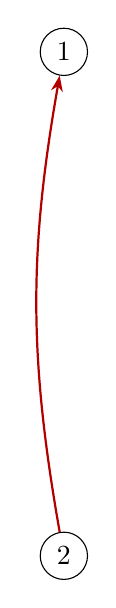
\begin{tikzpicture}[>={Stealth[length=2mm]}]
\node[draw,circle,minimum size=6mm,inner sep=0pt] (n0) at (0.00,3.20) {1};
\node[draw,circle,minimum size=6mm,inner sep=0pt] (n1) at (0.00,-3.20) {2};
\draw[->,red!70!black,thick] (n1) to[bend left=10] (n0);
\end{tikzpicture}
\end{center}
\noindent Solid: defeats. Dashed: supports. Dotted: one party's case is part of another's.
\begin{enumerate}
\item Tipton, on direct examination
\item Counsel, on cross-examination
\end{enumerate}
\begin{longtable}{@{}>{\raggedright\arraybackslash}p{0.3\textwidth} >{\raggedright\arraybackslash}p{0.3\textwidth} >{\raggedright\arraybackslash}p{0.3\textwidth}@{}}
\toprule
\textbf{From} & \textbf{To} & \textbf{Edge} \\
\midrule
\endhead
2 \emph{Counsel, on cross-examination} & 1 \emph{Tipton, on direct examination} & defeats \\
\bottomrule
\end{longtable}
\noindent The defeats are the cells of \texttt{grits\allowbreak{}Dispute\_\allowbreak{}defeats}, the supports the cells of \texttt{grits\allowbreak{}Dispute\_\allowbreak{}supports} and the parts the cells of \texttt{grits\allowbreak{}Dispute\_\allowbreak{}part\allowbreak{}Of}, each computed from the parties' premises and checked by the kernel. The attacks derived through support and through parts are reported, not counted: every verdict is computed from the defeats alone. Every derived attack is already a defeat.
\paragraph*{What the dispute decides}
\leavevmode\par
\par\medskip\noindent\textbf{\texttt{the\allowbreak{}Cross\allowbreak{}Examination\allowbreak{}Grounded}}\par\nobreak\noindent
Why the cross-examination prevails: nothing defeats it, so it is grounded from the first step, and it defeats the testimony, which nothing defends.

\paragraph{What the dispute forces is exactly \emph{Counsel, on cross-examination}.}
\begin{itemize}
\item Stage 1: \emph{Counsel, on cross-examination}.
\begin{itemize}
\item \emph{Counsel, on cross-examination} is defeated by nothing.
\end{itemize}
\item Nothing else is forced:
\begin{itemize}
\item \emph{Counsel, on cross-examination} defeats \emph{Tipton, on direct examination}, and nothing forced defeats \emph{Counsel, on cross-examination}.
\end{itemize}
\end{itemize}
\par\noindent\textbf{What this rests on.} The reasons state 1 defeat and 2 absences of defeat, each a cell of the defeat table, \texttt{grits\allowbreak{}Dispute\_\allowbreak{}defeats}, computed from the two parties' premises and checked by the kernel. Whether an attack survives turns on the attacker's weakest link and on the rating of what it attacks, so a changed rating can change the verdict. The weakest links:
\begin{itemize}
\item \emph{Tipton, on direct examination}, weakest at \emph{disputed}:
\begin{itemize}
\item Making his breakfast took Tipton five minutes --- \cite[11--12]{garland-novato-healthcare-2019}; \cite{launer-my-cousin-vinny-1992}
\end{itemize}
\item \emph{Counsel, on cross-examination}, weakest at \emph{well supported}:
\begin{itemize}
\item Regular grits take twenty minutes to cook --- \cite[11--12]{garland-novato-healthcare-2019}; \cite{launer-my-cousin-vinny-1992}
\item an inference step --- \cite[11--12]{garland-novato-healthcare-2019}; \cite{launer-my-cousin-vinny-1992}
\end{itemize}
\end{itemize}
\par\medskip\noindent\textbf{\texttt{the\_\allowbreak{}cross\_\allowbreak{}examination\_\allowbreak{}prevails}}\par\nobreak\noindent
\textbf{The cross-examination prevails.} However the dispute is resolved, the cross-examination is accepted and the testimony is not.

What this claims: given the record as rated — the five-minute breakfast contested, the step from the grits well supported — the five minutes cannot stand. What it does not claim: that twenty minutes passed, or anything about who shot the clerk.

{\small\begin{verbatim}
theorem the_cross_examination_prevails : Framework.grounded
    gritsDispute.defeats = {Side.cross}
-- axioms: propext, Classical.choice, Quot.sound
\end{verbatim}}
\par\medskip\noindent\textbf{\texttt{the\allowbreak{}Testimony\allowbreak{}Answered}}\par\nobreak\noindent
Why the testimony cannot be defended: the cross-examination defeats it, and nothing answers the cross-examination.

\paragraph{\emph{Tipton, on direct examination} cannot be defended: no admissible position holds it.}
\begin{itemize}
\item \emph{Counsel, on cross-examination} defeats \emph{Tipton, on direct examination}, and nothing defeats \emph{Counsel, on cross-examination}.
\end{itemize}
\par\noindent\textbf{What this rests on.} The reasons state 1 defeat and 2 absences of defeat, each a cell of the defeat table, \texttt{grits\allowbreak{}Dispute\_\allowbreak{}defeats}, computed from the two parties' premises and checked by the kernel. Whether an attack survives turns on the attacker's weakest link and on the rating of what it attacks, so a changed rating can change the verdict. The weakest links:
\begin{itemize}
\item \emph{Counsel, on cross-examination}, weakest at \emph{well supported}:
\begin{itemize}
\item Regular grits take twenty minutes to cook --- \cite[11--12]{garland-novato-healthcare-2019}; \cite{launer-my-cousin-vinny-1992}
\item an inference step --- \cite[11--12]{garland-novato-healthcare-2019}; \cite{launer-my-cousin-vinny-1992}
\end{itemize}
\item \emph{Tipton, on direct examination}, weakest at \emph{disputed}:
\begin{itemize}
\item Making his breakfast took Tipton five minutes --- \cite[11--12]{garland-novato-healthcare-2019}; \cite{launer-my-cousin-vinny-1992}
\end{itemize}
\end{itemize}
\par\medskip\noindent\textbf{\texttt{tiptons\_\allowbreak{}testimony\_\allowbreak{}cannot\_\allowbreak{}be\_\allowbreak{}defended}}\par\nobreak\noindent
\textbf{Tipton’s testimony cannot be defended.} No consistent position holding it answers the cross-examination.

{\small\begin{verbatim}
theorem tiptons_testimony_cannot_be_defended : ∀ (S : Set Side),
    Framework.Admissible gritsDispute.defeats S → Side.direct ∉ S
-- axioms: propext, Classical.choice, Quot.sound
\end{verbatim}}
\paragraph*{The dispute when Tipton said he was a fast cook}
\leavevmode\par
\par\medskip\noindent\textbf{\texttt{at\allowbreak{}The\allowbreak{}Fast\allowbreak{}Cook\allowbreak{}Node}}\par\nobreak\noindent
The parties as they stood when Tipton said he was a fast cook: the same packages, with the step from the grits rated as it was then.

{\small\begin{verbatim}
def atTheFastCookNode : Side → ArgumentPackage Claim :=
  fun x =>
    match x with
    | Side.direct => direct
    | Side.cross => crossAtTheFastCook
\end{verbatim}}
\par\medskip\noindent\textbf{\texttt{at\allowbreak{}The\allowbreak{}Fast\allowbreak{}Cook\allowbreak{}Dispute}}\par\nobreak\noindent
The dispute at the fast cook.

{\small\begin{verbatim}
def atTheFastCookDispute : Dispute Claim Side :=
  { node := atTheFastCookNode,
    consistent := atTheFastCookDispute._proof_3,
    sound := atTheFastCookDispute._proof_4,
    rated := atTheFastCookDispute._proof_5 }
\end{verbatim}}
\par\medskip\noindent\textbf{\texttt{fast\allowbreak{}Cook\allowbreak{}Defeats}}\par\nobreak\noindent
The defeats at the fast cook, as a table: a standoff.

{\small\begin{verbatim}
def fastCookDefeats : Side → Side → Prop :=
  fun x x_1 =>
    match x, x_1 with
    | Side.cross, Side.direct => True
    | Side.direct, Side.cross => True
    | x, x_2 => False
\end{verbatim}}
\par\medskip\noindent\textbf{\texttt{inst\allowbreak{}Decidable\allowbreak{}Rel\allowbreak{}Side\allowbreak{}Fast\allowbreak{}Cook\allowbreak{}Defeats}}\par\nobreak\noindent
The table is finite, so membership in it is decidable.

{\small\begin{verbatim}
def instDecidableRelSideFastCookDefeats : DecidableRel fastCookDefeats :=
  fun i j =>
    Side.casesOn (motive := fun t =>
      i = t → Decidable (fastCookDefeats i j)) i
      (fun h =>
        ⋯ ▸
          Side.casesOn (motive := fun t =>
            j = t → Decidable (fastCookDefeats Side.direct j)) j
            (fun h => ⋯ ▸ id inferInstance) (fun h => ⋯ ▸ id inferInstance) ⋯)
      (fun h =>
        ⋯ ▸
          Side.casesOn (motive := fun t =>
            j = t → Decidable (fastCookDefeats Side.cross j)) j
            (fun h => ⋯ ▸ id inferInstance) (fun h => ⋯ ▸ id inferInstance) ⋯)
      ⋯
\end{verbatim}}
\par\medskip\noindent\textbf{\texttt{fast\allowbreak{}Cook\allowbreak{}Strength}}\par\nobreak\noindent
Each side’s weakest link at the fast cook: \texttt{disputed} for both.

{\small\begin{verbatim}
def fastCookStrength : Side → ℕ :=
  fun x => 0
\end{verbatim}}
\par\medskip\noindent\textbf{\texttt{at\allowbreak{}The\allowbreak{}Fast\allowbreak{}Cook\allowbreak{}Node\_\allowbreak{}strength}}\par\nobreak\noindent
Each side’s weakest link at the fast cook, as its package computes it.

{\small\begin{verbatim}
theorem atTheFastCookNode_strength : ∀ (i : Side), (atTheFastCookNode
    i).strength = fastCookStrength i
-- axioms: propext
\end{verbatim}}
\par\medskip\noindent\textbf{\texttt{at\allowbreak{}The\allowbreak{}Fast\allowbreak{}Cook\allowbreak{}Dispute\_\allowbreak{}defeats}}\par\nobreak\noindent
\textbf{Who defeated whom at the fast cook}, all four pairs: a standoff. With both weakest links \texttt{disputed}, each side’s attacks on the other are defeats. Every cell is computed by \texttt{Horn.defeats?} and checked by the kernel.

{\small\begin{verbatim}
theorem atTheFastCookDispute_defeats : ∀ (i j : Side),
    atTheFastCookDispute.defeats i j ↔ fastCookDefeats i j
-- axioms: propext, Classical.choice, Quot.sound
\end{verbatim}}
\par\medskip\noindent\textbf{\texttt{at\allowbreak{}The\allowbreak{}Fast\allowbreak{}Cook\allowbreak{}Finite}}\par\nobreak\noindent
The dispute at the fast cook, in the form the verdict solver computes with.

{\small\begin{verbatim}
def atTheFastCookFinite : Solver.Finite atTheFastCookDispute.defeats :=
  { parties := [Side.direct, Side.cross],
    complete := gritsFinite._proof_1,
    defeats := fun i j => decide (fastCookDefeats i j),
    spec := atTheFastCookFinite._proof_1 }
\end{verbatim}}
\par\medskip\noindent\textbf{\texttt{at\allowbreak{}The\allowbreak{}Fast\allowbreak{}Cook\allowbreak{}Undecided}}\par\nobreak\noindent
Why nothing was decided at the fast cook: each side had a defeater.

\paragraph{Nothing prevails outright: every party is defeated by another.}
\begin{itemize}
\item \emph{Counsel, when Tipton said he was a fast cook} defeats \emph{Tipton, on direct examination}.
\item \emph{Tipton, on direct examination} defeats \emph{Counsel, when Tipton said he was a fast cook}.
\end{itemize}
\par\noindent\textbf{What this rests on.} The reasons state 2 defeats and 0 absences of defeat, each a cell of the defeat table, \texttt{at\allowbreak{}The\allowbreak{}Fast\allowbreak{}Cook\allowbreak{}Dispute\_\allowbreak{}defeats}, computed from the two parties' premises and checked by the kernel. Whether an attack survives turns on the attacker's weakest link and on the rating of what it attacks, so a changed rating can change the verdict. The weakest links:
\begin{itemize}
\item \emph{Counsel, when Tipton said he was a fast cook}, weakest at \emph{disputed}:
\begin{itemize}
\item an inference step --- \cite[11--12]{garland-novato-healthcare-2019}; \cite{launer-my-cousin-vinny-1992}
\end{itemize}
\item \emph{Tipton, on direct examination}, weakest at \emph{disputed}:
\begin{itemize}
\item Making his breakfast took Tipton five minutes --- \cite[11--12]{garland-novato-healthcare-2019}; \cite{launer-my-cousin-vinny-1992}
\end{itemize}
\end{itemize}
\par\medskip\noindent\textbf{\texttt{at\_\allowbreak{}the\_\allowbreak{}fast\_\allowbreak{}cook\_\allowbreak{}nothing\_\allowbreak{}was\_\allowbreak{}decided}}\par\nobreak\noindent
\textbf{When Tipton said he was a fast cook, nothing was decided.} He had granted the grounds of the step from the grits and denied its conclusion, so the step was \texttt{disputed}, and neither side was the stronger.

What this claims: that the twenty minutes alone did not settle it. What settled it was the witness’s withdrawing his denial (\texttt{the\_\allowbreak{}cross\_\allowbreak{}examination\_\allowbreak{}prevails}).

{\small\begin{verbatim}
theorem at_the_fast_cook_nothing_was_decided : Framework.grounded
    atTheFastCookDispute.defeats = ∅
-- axioms: propext, Classical.choice, Quot.sound
\end{verbatim}}
\par\medskip\noindent\textbf{\texttt{at\allowbreak{}The\allowbreak{}Fast\allowbreak{}Cook\allowbreak{}The\allowbreak{}Testimony\allowbreak{}Stood}}\par\nobreak\noindent
Why the testimony could still be defended at the fast cook: it answered the cross-examination itself.

\paragraph{\emph{Tipton, on direct examination} is accepted on some resolution.}
\begin{itemize}
\item A position holding \emph{Tipton, on direct examination} can be held.
\item \emph{Tipton, on direct examination} does not defeat itself, and answers each attack on it:
\begin{itemize}
\item \emph{Counsel, when Tipton said he was a fast cook} defeats \emph{Tipton, on direct examination}, and \emph{Tipton, on direct examination} defeats \emph{Counsel, when Tipton said he was a fast cook}.
\end{itemize}
\end{itemize}
\par\noindent\textbf{What this rests on.} The reasons state 2 defeats and 1 absence of defeat, each a cell of the defeat table, \texttt{at\allowbreak{}The\allowbreak{}Fast\allowbreak{}Cook\allowbreak{}Dispute\_\allowbreak{}defeats}, computed from the two parties' premises and checked by the kernel. Whether an attack survives turns on the attacker's weakest link and on the rating of what it attacks, so a changed rating can change the verdict. The weakest links:
\begin{itemize}
\item \emph{Tipton, on direct examination}, weakest at \emph{disputed}:
\begin{itemize}
\item Making his breakfast took Tipton five minutes --- \cite[11--12]{garland-novato-healthcare-2019}; \cite{launer-my-cousin-vinny-1992}
\end{itemize}
\item \emph{Counsel, when Tipton said he was a fast cook}, weakest at \emph{disputed}:
\begin{itemize}
\item an inference step --- \cite[11--12]{garland-novato-healthcare-2019}; \cite{launer-my-cousin-vinny-1992}
\end{itemize}
\end{itemize}
\par\medskip\noindent\textbf{\texttt{at\_\allowbreak{}the\_\allowbreak{}fast\_\allowbreak{}cook\_\allowbreak{}tiptons\_\allowbreak{}testimony\_\allowbreak{}could\_\allowbreak{}be\_\allowbreak{}defended}}\par\nobreak\noindent
\textbf{At the fast cook, Tipton’s testimony could still be defended}: holding it, he answered the cross-examination’s attack with his own.

{\small\begin{verbatim}
theorem at_the_fast_cook_tiptons_testimony_could_be_defended :
    Framework.CredulouslyAccepted atTheFastCookDispute.defeats Side.direct
-- axioms: propext, Classical.choice, Quot.sound
\end{verbatim}}

\bibliographystyle{plain}
\bibliography{references}
\end{document}
